\chapter{Cromatina e epigenética}\label{ch:b3:chromatin-epigenetics}

Dois camundongos da mesma ninhada, geneticamente idênticos até a
última base, estão lado a lado: um é magro e pardo, o outro é gordo e
amarelo, e ficará diabético. Uma gata de pelagem tricolor exibe
manchas alaranjadas e pretas embora cada célula de sua pele carregue
os mesmos dois cromossomos X. Uma criança herda o mesmo trecho
deletado do cromossomo 15 que outra criança, e uma tem a síndrome de
Prader--Willi enquanto a outra tem a síndrome de Angelman --- a
diferença está apenas em de qual dos pais veio a deleção. Nada disso
está escrito na sequência do DNA. Está escrito \emph{sobre} ela: no
modo como dois metros de DNA são acondicionados num núcleo de dez
micrômetros, nos pequenos grupos químicos ligados às proteínas de
empacotamento e às próprias citosinas, e na maquinaria que copia essas
marcas de uma célula para suas filhas. Este capítulo trata dessa
segunda camada de informação, de seus portadores moleculares e dos
limites honestos daquilo que ela consegue lembrar.

\section{Cromatina: o DNA num carretel}

\begin{definition}[Nucleossomo e cromatina]\label{def:b3:chromatin-epigenetics:nucleosome}
\index{nucleossomo}\index{cromatina}\index{histona}\index{eucromatina}\index{heterocromatina}
A \emph{cromatina} é o complexo do DNA com proteínas sob a forma do
qual o genoma existe num núcleo eucarionte. Sua unidade de repetição é
o \emph{nucleossomo}: \qty{147}{bp} de DNA enrolados em $1.65$ voltas
levógiras em torno de um octâmero de \emph{histonas} --- duas cópias
de cada uma das proteínas pequenas e muito básicas H2A, H2B, H3 e H4
--- seguidos de um \emph{ligante} de \qtyrange{20}{60}{bp} até o
nucleossomo seguinte. Uma quinta histona, a H1, liga-se ao ligante
onde ele entra e sai do cerne e ajuda as contas a se empacotarem umas
contra as outras. Cada histona do cerne tem uma \emph{cauda}
amino-terminal não estruturada, de umas \numrange{20}{40} resíduos,
que se projeta para fora da partícula. A cromatina que se cora
fracamente, é frouxamente empacotada e é transcrita é a
\emph{eucromatina}; a cromatina densamente empacotada, de replicação
tardia e em larga medida silenciosa, nos centrômeros, nos telômeros e
nas sequências repetidas, é a \emph{heterocromatina}.
\end{definition}

\begin{proof}[Evidência]
Hewish e Burgoyne (1973) digeriram núcleos de fígado de rato com uma
nuclease endógena e constataram que o DNA saía não como um rastro
contínuo, mas como uma escada de fragmentos cujos comprimentos eram
múltiplos de cerca de \qty{200}{bp}: o DNA estava protegido em
intervalos regulares e era cortado apenas entre eles. Kornberg (1974)
mostrou que a unidade protegida era uma partícula de oito \omterm{def:b3:chromatin-epigenetics:nucleosome}{histonas} com
cerca de \qty{200}{bp}, e micrografias eletrônicas de \omterm{def:b3:chromatin-epigenetics:nucleosome}{cromatina}
delicadamente espalhada mostraram as ``contas num colar''. Luger e
colaboradores (1997) resolveram a estrutura cristalográfica da
partícula do cerne a \qty{2.8}{\angstrom}: \qty{147}{bp}, um octâmero
com as caudas passando por entre os giros do DNA.
\end{proof}

\begin{omfigure}
\begin{tikzpicture}[every node/.style={font=\scriptsize}, >=stealth]
  % beads on a string
  \foreach \x/\y in {0/0, 2.2/0.5, 4.4/0, 6.6/0.5, 8.8/0} {
    \fill[omDef!30] (\x,\y) circle (0.42);
    \draw[very thick, omThm!70!black] (\x,\y) circle (0.5);
  }
  \draw[very thick, omThm!70!black] (-1.1,-0.1) -- (0-0.47,-0.17);
  \draw[very thick, omThm!70!black] (0.47,-0.17) -- (2.2-0.47,0.33);
  \draw[very thick, omThm!70!black] (2.67,0.33) -- (4.4-0.47,-0.17);
  \draw[very thick, omThm!70!black] (4.87,-0.17) -- (6.6-0.47,0.33);
  \draw[very thick, omThm!70!black] (7.07,0.33) -- (8.8-0.47,-0.17);
  \draw[very thick, omThm!70!black] (9.27,-0.17) -- (10.4,-0.1);
  % tails
  \foreach \x/\y in {0/0, 4.4/0, 8.8/0} { \draw[omProp, thick] (\x,\y+0.5) .. controls (\x-0.2,\y+0.9) .. (\x+0.1,\y+1.15); \draw[omProp, thick] (\x,\y-0.5) .. controls (\x+0.2,\y-0.9) .. (\x-0.1,\y-1.15); }
  \foreach \x/\y in {2.2/0.5, 6.6/0.5} { \draw[omProp, thick] (\x,\y+0.5) .. controls (\x-0.2,\y+0.9) .. (\x+0.1,\y+1.15); }
  % H1
  \fill[omMeth!70!black] (1.55,0.05) circle (0.12); \fill[omMeth!70!black] (5.95,0.05) circle (0.12);
  % labels
  \node[above, align=center] at (2.2,1.75) {caudas das histonas\\(acetilação, metilação)};
  \node[below, align=center] at (4.4,-1.35) {partícula do cerne: octâmero\\$+$ \qty{147}{bp}, $1.65$ voltas};
  \node[below, align=center] at (7.7,-0.55) {DNA ligante\\\qtyrange{20}{60}{bp}};
  \node[below] at (5.95,-0.1) {H1};
  \draw[<->] (-0.5,-2.2) -- (2.2-0.5,-2.2) node[midway, below] {repetição $\approx \qty{200}{bp}$, \qty{11}{nm}};
  \draw[gray] (-0.5,-1.95) -- (-0.5,-2.35); \draw[gray] (1.7,-1.95) -- (1.7,-2.35);
\end{tikzpicture}

{\small A fibra de \qty{10}{nm}: cernes de \omterm{def:b3:chromatin-epigenetics:nucleosome}{nucleossomo} (azul) sobre um
DNA contínuo (vermelho), cada conta um octâmero de \omterm{def:b3:chromatin-epigenetics:nucleosome}{histonas} com suas
caudas (laranja) projetadas para fora, a \omterm{def:b3:chromatin-epigenetics:nucleosome}{histona} ligante H1 (verde) no
ponto de entrada e saída. Cerca de seis \omterm{def:b3:chromatin-epigenetics:nucleosome}{nucleossomos} ocupam o
comprimento que \qty{1200}{bp} de DNA nu ocupariam.}
\end{omfigure}

\begin{omfigure}
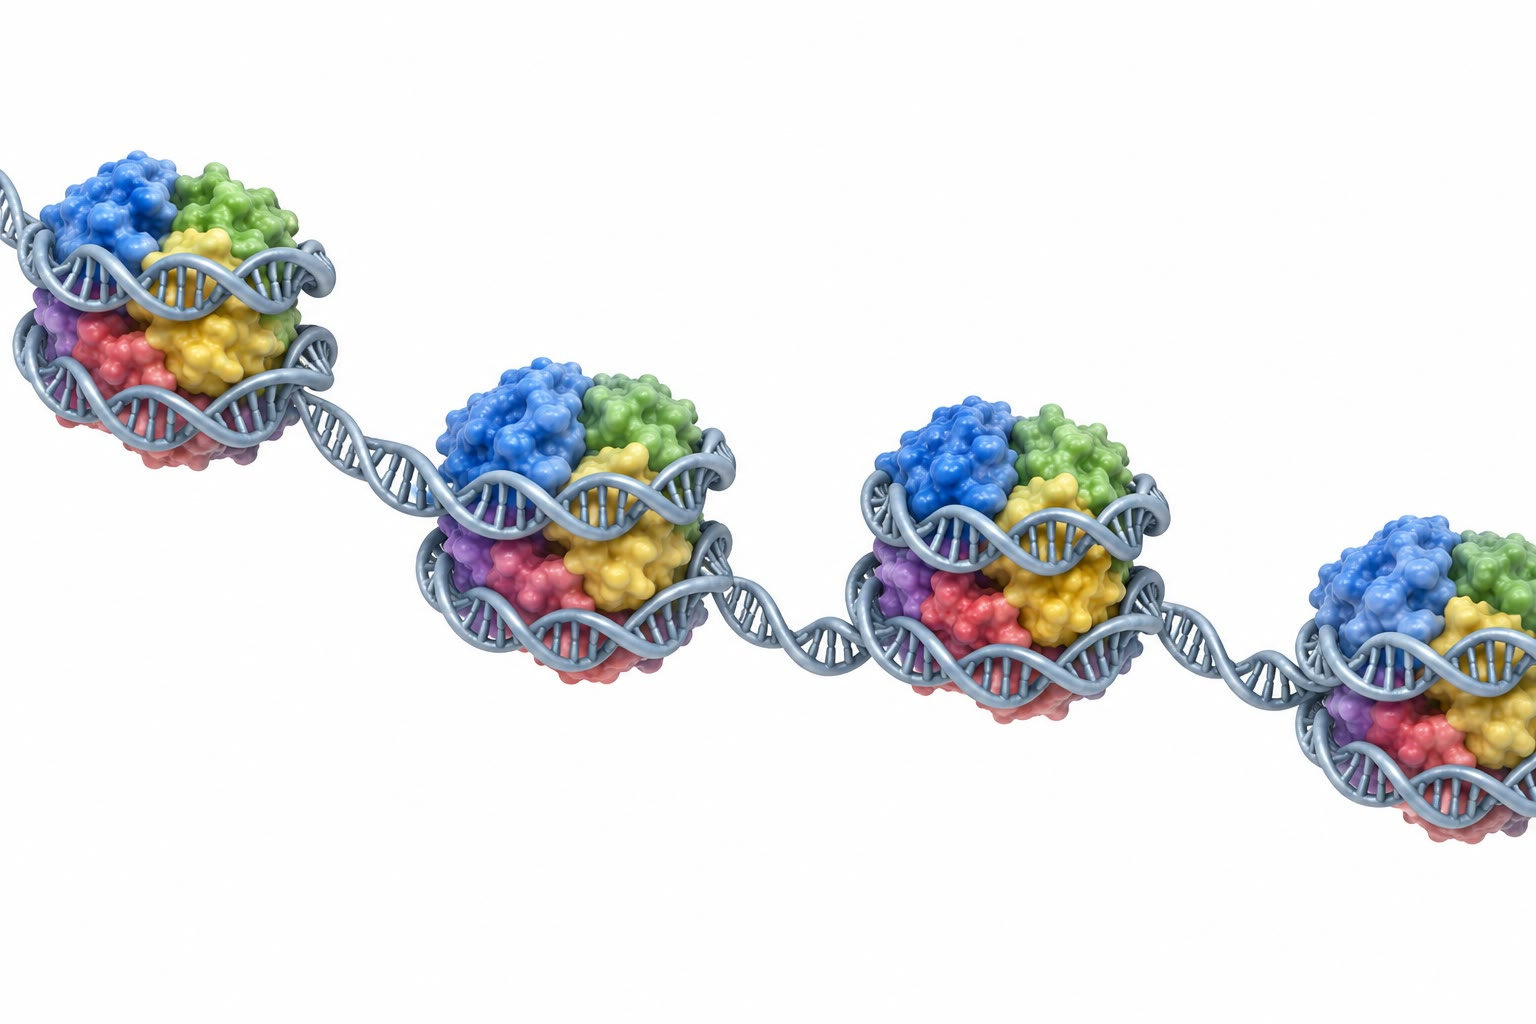
\includegraphics[width=0.6\linewidth]{images/book5/ai/b5-01-nucleosomes.jpg}

{\small A \omterm{def:b3:chromatin-epigenetics:nucleosome}{cromatina} na escala molecular: a dupla-hélice enrolada em
torno de cernes sucessivos de \omterm{def:b3:chromatin-epigenetics:nucleosome}{histonas}, as ``contas num colar'' que a
escada da nuclease revelou.}
\end{omfigure}

\begin{proposition}[Níveis de compactação]\label{prop:b3:chromatin-epigenetics:compaction}
\index{razão de empacotamento}\index{alça de cromatina}\index{domínio de associação topológica}
A \emph{\omterm{prop:b3:chromatin-epigenetics:compaction}{razão de empacotamento}} de uma estrutura de \omterm{def:b3:chromatin-epigenetics:nucleosome}{cromatina} é o
comprimento do DNA que ela contém dividido pelo comprimento da
estrutura. O enrolamento na fibra de \qty{10}{nm} dá uma razão de
cerca de $6$: os \qty{68}{nm} de uma repetição de \qty{200}{bp} são
comprimidos numa única conta de \qty{11}{nm}. No núcleo interfásico a
fibra não se enrola numa fibra regular mais grossa, como os livros por
muito tempo a desenharam, mas se dobra em \emph{alças} de dezenas a
centenas de quilobases mantidas em suas bases por complexos de coesina
em forma de anel e pela proteína ligadora de DNA CTCF; as alças se
agrupam em \emph{\omterm{prop:b3:chromatin-epigenetics:compaction}{domínios de associação topológica}} (TADs) de cerca de
uma megabase, dentro dos quais um gene encontra seus reguladores muito
mais vezes do que encontra qualquer coisa de fora. Um cromossomo
mitótico, o estado mais compacto, tem uma \omterm{prop:b3:chromatin-epigenetics:compaction}{razão de empacotamento}
próxima de \num{10000}: os \qty{4}{cm} de DNA de um cromossomo humano
médio são dobrados num bastão de \qty{4}{\micro m} de comprimento.
\end{proposition}

\begin{example}[Dois metros em dez micrômetros]\label{ex:b3:chromatin-epigenetics:two-metres}
Um núcleo diploide humano contém $6.4\times 10^{9}$ pares de bases. A
\qty{0.34}{nm} por par de bases isso dá \qty{2.2}{m} de dupla-hélice,
num núcleo de cerca de \qty{10}{\micro m} de diâmetro. Tudo isso é
acondicionado em $6.4\times 10^{9}/200 \approx 3.2\times 10^{7}$
\omterm{def:b3:chromatin-epigenetics:nucleosome}{nucleossomos}, cada um carregando cerca de \qty{108}{kDa} de \omterm{def:b3:chromatin-epigenetics:nucleosome}{histonas}
contra \qty{96}{kDa} de DNA (\qty{147}{bp} a \qty{650}{Da} por par): o
núcleo contém, em massa, aproximadamente tanta \omterm{def:b3:chromatin-epigenetics:nucleosome}{histona} quanto DNA. O
próprio DNA, tratado como um cilindro de \qty{2}{nm} de diâmetro, tem
um volume de apenas cerca de \qty{7}{\micro m^3}, uns \qty{1}{\%} de
um núcleo esférico de raio \qty{5}{\micro m}; o problema do
empacotamento é de emaranhamento e de acesso, não de espaço.
\end{example}

\section{O código das histonas}

\begin{definition}[Modificações das histonas]\label{def:b3:chromatin-epigenetics:histone-code}
\index{código das histonas}\index{acetilação}\index{metilação de histonas}\index{escritor}\index{leitor}\index{apagador}
Os resíduos das caudas das \omterm{def:b3:chromatin-epigenetics:nucleosome}{histonas} sofrem modificações covalentes:
\emph{acetilação} de lisinas (que neutraliza sua carga positiva e
afrouxa o aperto sobre o DNA), \emph{metilação} de lisinas e argininas
(um, dois ou três grupos metila, sem mudança de carga), fosforilação
de serinas, ubiquitinação de lisinas. Uma modificação é nomeada pela
\omterm{def:b3:chromatin-epigenetics:nucleosome}{histona}, pelo resíduo e pelo grupo: H3K4me3 é a \omterm{def:b3:chromatin-epigenetics:nucleosome}{histona} H3, lisina 4,
trimetilada; H3K27ac é a H3 com a lisina 27 acetilada. O \emph{código
das \omterm{def:b3:chromatin-epigenetics:nucleosome}{histonas}} é a correlação entre combinações de marcas e o estado do
gene subjacente: H3K4me3 e H3K27ac em promotores e intensificadores
ativos, H3K36me3 ao longo dos corpos dos genes transcritos, H3K9me3 na
\omterm{def:b3:chromatin-epigenetics:nucleosome}{heterocromatina} constitutiva, H3K27me3 em genes silenciados durante o
desenvolvimento. As enzimas que acrescentam uma marca são
\emph{escritores} (acetiltransferases de \omterm{def:b3:chromatin-epigenetics:nucleosome}{histonas}, HATs;
metiltransferases), as que a removem são \emph{apagadores}
(desacetilases de \omterm{def:b3:chromatin-epigenetics:nucleosome}{histonas}, HDACs; desmetilases), e as proteínas que
se ligam a uma marca e agem sobre ela são \emph{leitores}: um
\emph{bromodomínio} liga acetil-lisina, um \emph{cromodomínio}
metil-lisina.
\end{definition}

\begin{proposition}[As marcas são lidas, não apenas sentidas]\label{prop:b3:chromatin-epigenetics:readers}
\index{HP1}\index{Polycomb}\index{PRC2}\index{Trithorax}
A \omterm{def:b3:chromatin-epigenetics:histone-code}{acetilação} age em parte por eletrostática --- uma cauda acetilada
segura seu DNA com menos força e a fibra se abre --- mas a maioria das
marcas age recrutando \omterm{def:b3:chromatin-epigenetics:histone-code}{leitores}. A H3K9me3 é ligada pelo cromodomínio
da \emph{proteína de \omterm{def:b3:chromatin-epigenetics:nucleosome}{heterocromatina} HP1}, que dimeriza, faz ponte
entre \omterm{def:b3:chromatin-epigenetics:nucleosome}{nucleossomos} vizinhos e recruta a própria metiltransferase
(SUV39H) que escreve H3K9me3 no \omterm{def:b3:chromatin-epigenetics:nucleosome}{nucleossomo} seguinte: a marca se
propaga ao longo da fibra até encontrar uma fronteira, e compacta o
que cobre. A H3K27me3 é escrita pelo \emph{complexo repressor Polycomb
2} (PRC2, subunidade catalítica EZH2), lida pelo PRC1, que
ubiquitina a H2A e compacta a fibra, e o complexo é ele próprio
estimulado pela marca que produz; o grupo de proteínas
\emph{Trithorax} escreve a H3K4me3 oposta e mantém ligados os genes do
desenvolvimento de um dado tipo celular. Cada uma dessas alças --- o
\omterm{def:b3:chromatin-epigenetics:histone-code}{leitor} recruta o \omterm{def:b3:chromatin-epigenetics:histone-code}{escritor} --- é uma retroalimentação positiva que
permite a um estado manter-se depois de estabelecido, que é do que uma
marca hereditária precisa.
\end{proposition}

\begin{omfigure}
\begin{tikzpicture}[every node/.style={font=\scriptsize}, >=stealth]
  % nucleosomes with tails
  \foreach \x in {0,2,4,6} { \draw[thick, omDef, fill=omDef!20] (\x,0) circle (0.45); \draw[omProp, thick] (\x,0.45) -- (\x,1.15); }
  % marks
  \fill[omThm] (2,1.15) circle (0.11); \fill[omThm] (4,1.15) circle (0.11);
  \fill[omMeth!80!black] (0,1.15) circle (0.11);
  \node[left] at (-0.5,1.15) {ac};
  \node[right, align=left] at (6.15,1.15) {me3};
  % HP1 reader
  \draw[thick, fill=omExo!30] (2.6,1.7) ellipse (0.5 and 0.25); \node at (2.6,1.7) {leitor};
  \draw[thick, fill=omExo!30] (4.2,2.35) ellipse (0.55 and 0.25); \node at (4.2,2.35) {escritor};
  \draw[->, thick] (2.9,1.9) -- (3.75,2.2);
  \draw[->, thick, omThm] (4.6,2.15) .. controls (5.6,2.0) and (6.1,1.8) .. (6.05,1.3);
  \node[right, align=left, font=\scriptsize] at (6.6,2.0) {propaga-se ao\\nucleossomo seguinte};
  \draw[->, thick, gray] (2.2,1.3) -- (2.45,1.5);
  % eraser
  \draw[thick, fill=omExo!30] (0.6,2.2) ellipse (0.5 and 0.25); \node at (0.6,2.2) {apagador};
  \draw[->, thick, omMeth!80!black] (0.3,2.0) -- (0.05,1.35);
  % DNA
  \draw[very thick, omThm!70!black] (-0.9,-0.3) -- (-0.45,-0.05) (0.45,-0.05) -- (1.55,-0.05) (2.45,-0.05) -- (3.55,-0.05) (4.45,-0.05) -- (5.55,-0.05) (6.45,-0.05) -- (7.2,-0.3);
  \node[below, align=center] at (0,-0.6) {aberta: o grupo acetila\\remove uma carga};
  \node[below, align=center] at (5,-0.6) {fechada: H3K9me3 lida pela HP1,\\que recruta a metilase da K9};
\end{tikzpicture}

{\small A lógica escritor--leitor--apagador. Um \omterm{def:b3:chromatin-epigenetics:histone-code}{leitor} ligado a uma
marca num \omterm{def:b3:chromatin-epigenetics:nucleosome}{nucleossomo} recruta o \omterm{def:b3:chromatin-epigenetics:histone-code}{escritor} que põe a mesma marca no
seguinte, de modo que o estado se propaga e se copia; os \omterm{def:b3:chromatin-epigenetics:histone-code}{apagadores} se
opõem a isso. Os grupos acetila (verde) abrem a fibra; a H3K9me3
(vermelho) a fecha.}
\end{omfigure}

\begin{method}[Imunoprecipitação da cromatina (ChIP)]\label{met:b3:chromatin-epigenetics:chip}
\index{ChIP}\index{imunoprecipitação da cromatina}
Para mapear onde uma marca ou uma proteína se assenta no genoma: (1)
faça a ligação cruzada das proteínas ao DNA em células vivas com
formaldeído; (2) fragmente a \omterm{def:b3:chromatin-epigenetics:nucleosome}{cromatina} em pedaços de algumas centenas
de pares de bases; (3) precipite os fragmentos com um anticorpo contra
a marca (digamos H3K27me3) preso a esferas; (4) desfaça as ligações
cruzadas e purifique o DNA; (5) sequencie-o (ChIP-seq) e conte as
leituras ao longo do genoma: os picos são os lugares onde a marca
estava. Um controle de DNA de entrada sem anticorpo fixa o ruído de
fundo. A resolução é a dos fragmentos, cerca de um \omterm{def:b3:chromatin-epigenetics:nucleosome}{nucleossomo}.
\end{method}

\begin{remark}[Código ou correlação]\label{rem:b3:chromatin-epigenetics:code}
A palavra ``código'' exagera o caso. Muitas marcas são consequências
da transcrição, e não causas dela (a H3K36me3 é depositada por uma
metiltransferase que viaja com a polimerase), e retirar um \omterm{def:b3:chromatin-epigenetics:histone-code}{escritor}
muitas vezes muda a expressão bem menos do que a distribuição da marca
sugere. O que está bem estabelecido é que algumas poucas marcas ---
H3K9me3, H3K27me3 e a \omterm{def:b3:chromatin-epigenetics:methylation}{metilação do DNA}, adiante --- carregam um
silenciamento autopropagante que sobrevive ao sinal que o instaurou.
\end{remark}

\section{A metilação do DNA e a cópia de uma marca}

\begin{definition}[Metilação do DNA]\label{def:b3:chromatin-epigenetics:methylation}
\index{metilação do DNA}\index{CpG}\index{ilha CpG}\index{DNMT1}\index{metilação de manutenção}\index{metilação de novo}
Nos vertebrados um grupo metila é acrescentado ao carbono 5 da
citosina quase somente no dinucleotídeo \emph{CpG} (um C seguido de um
G na mesma fita), uma sequência que é seu próprio complemento, de modo
que um CpG metilado costuma estar metilado nas duas fitas. Cerca de
\qtyrange{70}{80}{\%} dos CpGs de uma célula humana estão metilados, e
promotores metilados são silenciosos: os grupos metila são lidos por
proteínas ligadoras de metil-CpG (MeCP2, MBD1--4) que recrutam HDACs e
metilases da H3K9, e bloqueiam diretamente vários fatores de
transcrição. As exceções são as \emph{ilhas CpG}, trechos de cerca de
uma quilobase, ricos em G e C e em CpG, que se situam nos promotores
da maioria dos genes de manutenção e permanecem não metilados em
células normais. O grupo metila é escrito pelas \emph{DNA
metiltransferases}: a DNMT3A e a DNMT3B realizam a \emph{metilação de
novo} de sítios não metilados, e a \emph{DNMT1}, que prefere um CpG
hemimetilado --- uma fita metilada, a outra não ---, realiza a
\emph{metilação de manutenção} atrás da forquilha de replicação. A
remoção é passiva, por replicação sem manutenção, ou ativa, pelas
enzimas TET, que oxidam a 5-metilcitosina a 5-hidroximetilcitosina e
além, até que o reparo por excisão de bases a troque por uma citosina
comum.
\end{definition}

\begin{example}[Por que o genoma é pobre em CpG]\label{ex:b3:chromatin-epigenetics:cpg-deficit}
O genoma humano tem \qty{42}{\%} de G$+$C, de modo que, se as bases
fossem independentes, um \omterm{def:b3:chromatin-epigenetics:methylation}{CpG} ocorreria com a frequência
$0.21\times 0.21 \approx 0.044$, cerca de $2.8\times 10^{8}$ vezes no
genoma diploide.
O número observado é de cerca de $5.6\times 10^{7}$, um quinto disso.
A razão é a própria marca: uma citosina metilada que perde seu grupo
amino torna-se timina, uma base normal que o reparo não consegue
reconhecer como errada, ao passo que uma citosina não metilada se
desamina a uracila, que é excisada. Ao longo do tempo evolutivo os
\omterm{def:b3:chromatin-epigenetics:methylation}{CpGs} metilados mutaram em TpG e CpA, e só as ilhas não metiladas
conservaram seus \omterm{def:b3:chromatin-epigenetics:methylation}{CpGs}. A marca deixou sua assinatura na sequência.
\end{example}

\begin{theorem}[Manutenção de um estado de metilação ao longo das divisões]\label{thm:b3:chromatin-epigenetics:maintenance}
\index{memória epigenética}\index{cadeia de Markov!metilação}
Considere um único sítio \omterm{def:b3:chromatin-epigenetics:methylation}{CpG}, acompanhado ao longo de uma linhagem de
células. A cada divisão a citosina da fita nova é metilada com
probabilidade $\mu$ se a citosina da fita-molde está metilada
(eficiência de manutenção) e com probabilidade $\delta$ se não está
(taxa de novo). Seja $p_{n}$ a probabilidade de o sítio estar metilado
após $n$ divisões. Então
\[
p_{n+1} = \mu\, p_{n} + \delta\,(1 - p_{n}),
\qquad
p_{n} = p^{*} + (p_{0} - p^{*})\,(\mu - \delta)^{n},
\qquad
p^{*} = \frac{\delta}{1 - \mu + \delta}.
\]
Todo sítio deriva rumo ao mesmo equilíbrio $p^{*}$, qualquer que seja
seu estado inicial, e a memória do estado inicial decai
geometricamente com razão $\mu - \delta$. Uma marca é lembrada durante
cerca de $1/(1 - \mu + \delta)$ divisões; a memória fiel de uma
\emph{diferença} entre sítios exige, portanto, um $\mu$ muito próximo
de $1$ e um $\delta$ muito próximo de $0$, ou uma retroalimentação que
faça $\mu$ e $\delta$ dependerem do estado da vizinhança.
\end{theorem}
\begin{proof}
A recorrência é a lei da probabilidade total sobre os dois estados da
fita-molde. Seu ponto fixo resolve $p^{*} = \mu p^{*} + \delta(1 -
p^{*})$, o que dá $p^{*}(1 - \mu + \delta) = \delta$. Subtraindo a
equação do ponto fixo da recorrência, $p_{n+1} - p^{*} = (\mu -
\delta)(p_{n} - p^{*})$, que iterada dá a forma fechada. Como
$0 \le \delta \le \mu \le 1$, a razão $\mu - \delta$ está em $[0,1]$ e
o desvio encolhe; ele cai pela metade a cada $\ln 2 / (-\ln(\mu -
\delta)) \approx \ln 2/(1 - \mu + \delta)$ divisões quando $\mu -
\delta$ está perto de $1$.
\end{proof}

\begin{example}[Números]\label{ex:b3:chromatin-epigenetics:maintenance-numbers}
Os valores medidos em células de mamífero são $\mu \approx 0.99$ e
$\delta \approx 0.02$ por divisão num \omterm{def:b3:chromatin-epigenetics:methylation}{CpG} típico. Então $p^{*} =
0.02/0.03 \approx 0.67$, próximo da fração metilada de todo o genoma,
e $\mu - \delta = 0.97$: um sítio totalmente metilado entregue apenas
à maquinaria estaria a meio caminho de volta à média após $\ln 2 /
0.03 \approx 23$ divisões. Um promotor silenciado que permanece
silencioso durante as centenas de divisões de uma vida precisa,
portanto, de mais do que a \omterm{def:b3:chromatin-epigenetics:methylation}{DNMT1}: os \omterm{def:b3:chromatin-epigenetics:histone-code}{leitores} de \omterm{def:b3:chromatin-epigenetics:methylation}{metil-CpG} recrutam a
metilação da H3K9 e os \omterm{def:b3:chromatin-epigenetics:histone-code}{leitores} da H3K9 recrutam a DNMT3, de modo que
uma ilha densa de marcas eleva seu próprio $\mu$ rumo a $1$ e abaixa o
$\delta$ vizinho rumo a $0$. Inversamente, uma célula que perde a
\omterm{def:b3:chromatin-epigenetics:methylation}{DNMT1} perde a marca passivamente: com $\mu = \delta = 0$ a fração de
fitas metiladas cai pela metade a cada divisão.
\end{example}

\begin{omfigure}
\begin{tikzpicture}[every node/.style={font=\scriptsize}, >=stealth]
  % left: replication scheme
  \begin{scope}
    \draw[very thick, omThm!70!black] (0,1.2) -- (2.4,1.2); \draw[very thick, omThm!70!black] (0,0.9) -- (2.4,0.9);
    \foreach \x in {0.5,1.2,1.9} { \fill[omDef] (\x,1.2) circle (0.09); \fill[omDef] (\x,0.9) circle (0.09); }
    \node[above] at (1.2,1.3) {parental: as duas fitas metiladas};
    \draw[->, thick] (1.2,0.75) -- (1.2,0.15) node[midway, right] {replicação};
    \draw[very thick, omThm!70!black] (0,-0.1) -- (2.4,-0.1); \draw[very thick, gray] (0,-0.4) -- (2.4,-0.4);
    \foreach \x in {0.5,1.2,1.9} { \fill[omDef] (\x,-0.1) circle (0.09); \draw[omDef] (\x,-0.4) circle (0.09); }
    \node[left] at (-0.1,-0.25) {hemimetilado};
    \draw[->, thick] (1.2,-0.85) -- (1.2,-1.45) node[midway, right, align=left] {DNMT1, probabilidade $\mu$\\por sítio};
    \draw[very thick, omThm!70!black] (0,-1.7) -- (2.4,-1.7); \draw[very thick, gray] (0,-2.0) -- (2.4,-2.0);
    \foreach \x in {0.5,1.9} { \fill[omDef] (\x,-1.7) circle (0.09); \fill[omDef] (\x,-2.0) circle (0.09); }
    \fill[omDef] (1.2,-1.7) circle (0.09); \draw[omDef] (1.2,-2.0) circle (0.09);
    \node[below, align=center] at (1.2,-2.1) {restaurado, um sítio perdido:\\a fita nova da célula-filha};
  \end{scope}
  % right: decay plot
  \begin{scope}[xshift=5.0cm, yshift=-2.3cm]
  \begin{axis}[
    width=6.6cm, height=4.6cm, axis lines=left,
    xmin=0, xmax=100, ymin=0, ymax=1.05,
    xlabel={divisões $n$},
    xlabel style={font=\scriptsize, at={(axis description cs:0.5,-0.1)}, anchor=north},
    tick label style={font=\scriptsize}, xtick={0,25,50,75,100}, ytick={0,0.5,0.67,1},
    yticklabels={0,0.5,$p^{*}$,1}, clip=false,
  ]
  \addplot[very thick, omDef, domain=0:100, samples=60] {0.6667 + 0.3333*0.97^x};
  \addplot[very thick, omThm, domain=0:100, samples=60] {0.6667 - 0.6667*0.97^x};
  \addplot[dashed, gray, domain=0:100, samples=2] {0.6667};
  \addplot[thick, omMeth!80!black, domain=0:100, samples=60] {0.6667 + 0.3333*0.998^x};
  \node[font=\scriptsize] at (axis cs:-9,1.1) {$p_{n}$};
  \node[font=\scriptsize, omDef, anchor=south west] at (axis cs:45,0.82) {início metilado, $\mu = 0.99$};
  \node[font=\scriptsize, omThm, anchor=north west] at (axis cs:50,0.30) {início não metilado};
  \node[font=\scriptsize, omMeth!80!black, anchor=south west] at (axis cs:30,1.02) {com retroalimentação, $\mu = 0.999$};
  \end{axis}
  \end{scope}
\end{tikzpicture}

{\small À esquerda: a \omterm{def:b3:chromatin-epigenetics:methylation}{metilação de manutenção}. Após a replicação todo
\omterm{def:b3:chromatin-epigenetics:methylation}{CpG} está hemimetilado; a \omterm{def:b3:chromatin-epigenetics:methylation}{DNMT1} copia a marca para a fita nova com
probabilidade $\mu$ por sítio. À direita: o destino de um sítio ao
longo das divisões para $\mu = 0.99$, $\delta = 0.02$ (azul a partir
do estado metilado, vermelho a partir do não metilado) --- ambos
convergem para $p^{*} = 0.67$ --- e para um sítio cuja
retroalimentação de vizinhança eleva $\mu$ a $0.999$ (verde).}
\end{omfigure}

\begin{method}[Ler a metilação: sequenciamento por bissulfito]\label{met:b3:chromatin-epigenetics:bisulfite}
\index{sequenciamento por bissulfito}
O sequenciamento sozinho não enxerga um grupo metila. Trate o DNA
desnaturado com bissulfito de sódio: a citosina não metilada é
desaminada a uracila, que é lida como T depois da PCR, ao passo que a
5-metilcitosina fica protegida e continua sendo lida como C.
Sequencie o DNA convertido e compare-o com a referência: todo C que
continuou C estava metilado, todo C que virou T não estava. Feito para
todo o genoma (\omterm{met:b3:chromatin-epigenetics:bisulfite}{sequenciamento por bissulfito} do genoma inteiro), isso
dá o estado de metilação de cada um dos $2.8\times 10^{7}$ \omterm{def:b3:chromatin-epigenetics:methylation}{CpGs} de um
genoma haploide com resolução de uma base, como fração das células da
amostra.
\end{method}

\section{Inativação do X e imprinting genômico}

\begin{definition}[Inativação do cromossomo X]\label{def:b3:chromatin-epigenetics:x-inactivation}
\index{inativação do X}\index{corpúsculo de Barr}\index{Xist}\index{compensação de dose}
Nas fêmeas de mamífero um dos dois cromossomos X de cada célula
somática é silenciado transcricionalmente cedo no desenvolvimento, uma
forma de \emph{compensação de dose} que iguala a expressão dos genes
ligados ao X entre fêmeas XX e machos XY. O cromossomo silenciado é
compactado num corpo denso encostado no envoltório nuclear, o
\emph{corpúsculo de Barr}. A escolha de qual X silenciar é aleatória
no embrião propriamente dito e, uma vez feita, é herdada clonalmente
por todos os descendentes da célula. A inativação é iniciada pelo
\emph{Xist}, um RNA não codificante de \qty{17}{kb} transcrito a
partir do centro de inativação do X do cromossomo que será silenciado:
ele recobre esse cromossomo em cis, recruta o Polycomb (H3K27me3), a
variante de \omterm{def:b3:chromatin-epigenetics:nucleosome}{histona} macroH2A e, por fim, a \omterm{def:b3:chromatin-epigenetics:methylation}{metilação do DNA} dos
promotores, e daí em diante o silêncio é mantido sem que o Xist seja
necessário a cada divisão. Cerca de \qty{15}{\%} dos genes humanos
ligados ao X escapam da inativação, em parte ou por inteiro.
\end{definition}

\begin{proof}[Evidência]
Barr e Bertram (1949) notaram um corpo denso nos núcleos de neurônios
de gatas, mas não de gatos. Ohno (1959) mostrou que ele era um
cromossomo X inteiro, condensado. Lyon (1961) juntou as peças: as
fêmeas de camundongo heterozigóticas para genes de cor de pelagem
ligados ao X têm uma pelagem em mosaico, com manchas que expressam um
alelo ou o outro, de modo que cada mancha é um clone no qual um X,
sempre o mesmo, está silencioso; o mesmo vale para as manchas
alaranjadas e pretas de uma gata tartaruga ou tricolor, cujo gene
alaranjado é ligado ao X, e para as glândulas sudoríparas em mosaico
das mulheres portadoras de um alelo mutante de um gene ligado ao X. Um
gato tricolor macho é quase sempre XXY.
\end{proof}

\begin{omfigure}
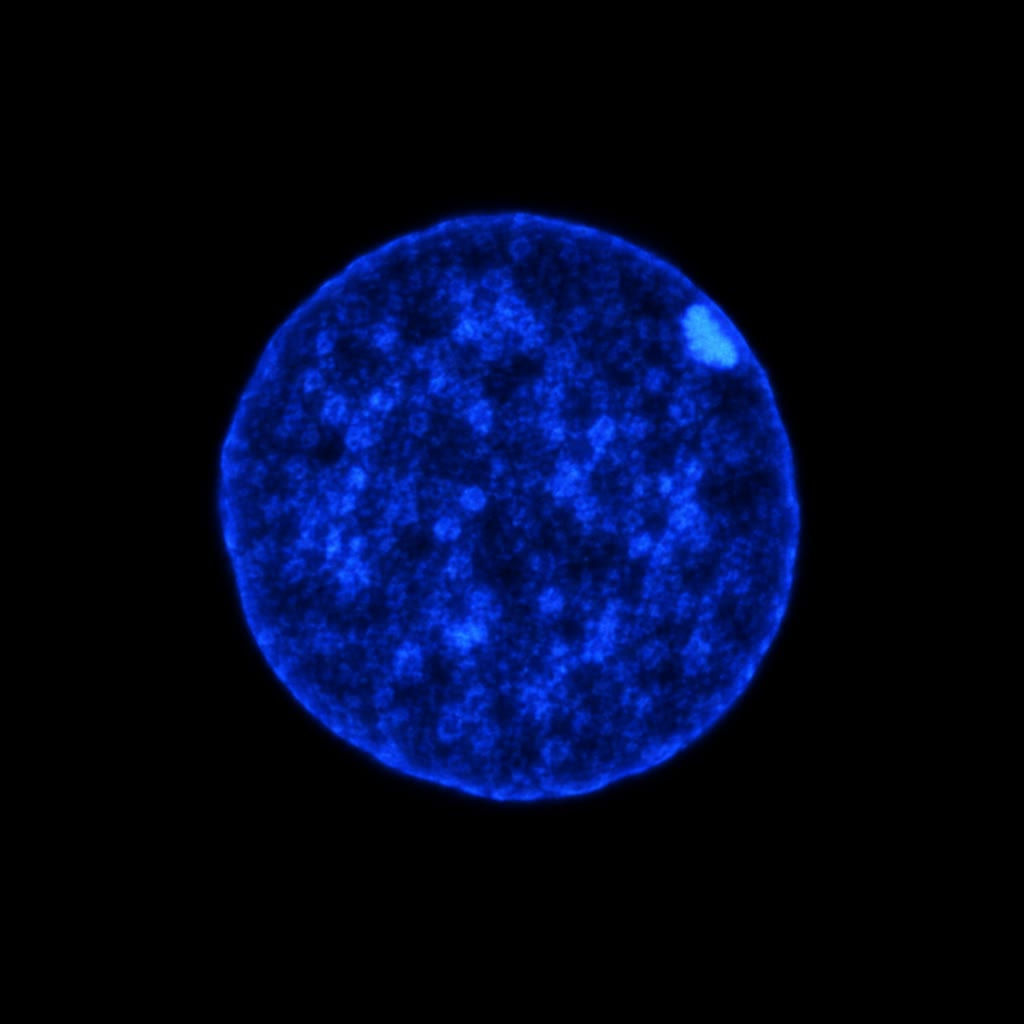
\includegraphics[width=0.42\linewidth]{images/book5/ai/b5-01-barr-body.jpg}\hspace{0.04\linewidth}
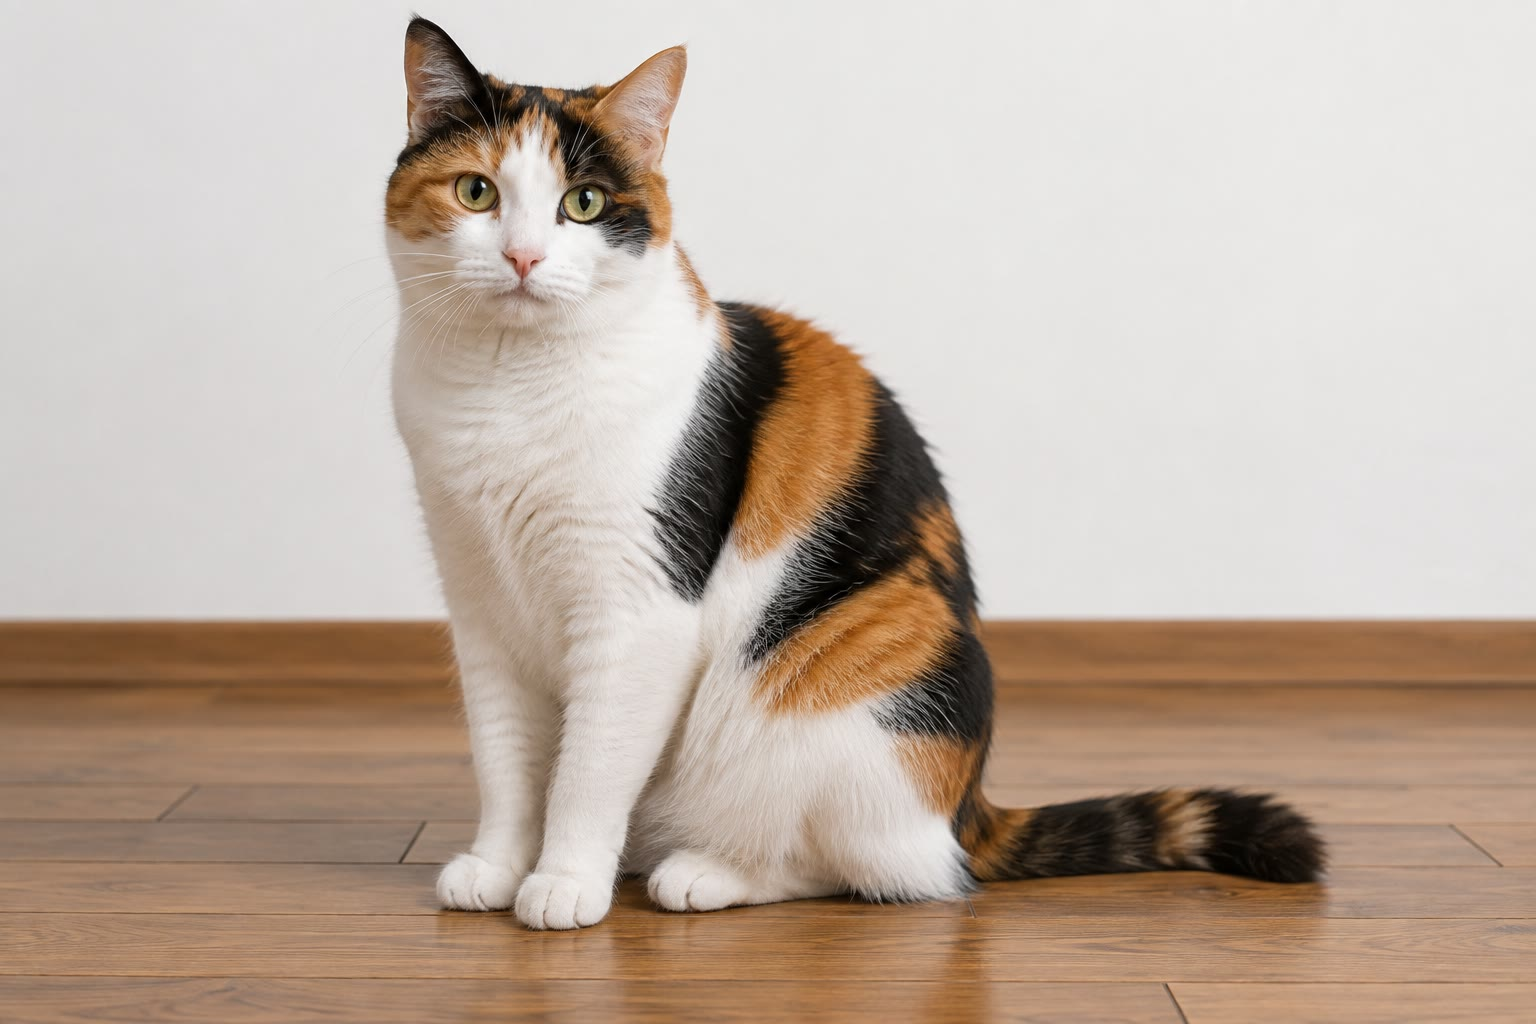
\includegraphics[width=0.5\linewidth]{images/book5/ai/b5-01-calico-cat.jpg}

{\small À esquerda: um núcleo feminino corado para DNA, com o X
inativo compacto --- o \omterm{def:b3:chromatin-epigenetics:x-inactivation}{corpúsculo de Barr} --- comprimido contra a
borda nuclear. À direita: uma gata tricolor. Cada mancha alaranjada ou
preta é um clone de células da pele que silenciaram o mesmo cromossomo
X; o branco é um gene de manchamento à parte, autossômico.}
\end{omfigure}

\begin{definition}[Imprinting genômico]\label{def:b3:chromatin-epigenetics:imprinting}
\index{imprinting genômico}\index{região controladora do imprinting}\index{dissomia uniparental}
Um gene está \emph{sob imprinting} quando apenas um de seus dois
alelos é expresso, e qual deles depende do genitor de que veio: alguns
genes são expressos só a partir da cópia paterna, outros só a partir
da materna. Os mamíferos têm uns \numrange{100}{200} genes sob
imprinting, agrupados, cada agrupamento governado por uma \emph{região
controladora do imprinting} (ICR) que está metilada num dos alelos
parentais e não no outro. A metilação é fixada na linhagem germinativa
--- um padrão nos espermatozoides, outro nos óvulos ---, apagada nas
células germinativas da geração seguinte e fixada de novo conforme o
sexo daquele indivíduo. Uma criança que recebe as duas cópias de um
cromossomo do mesmo genitor (\emph{dissomia uniparental}) tem,
portanto, a dose errada dos genes sob imprinting nele, embora sua
sequência seja inteiramente normal.
\end{definition}

\begin{proof}[Evidência]
McGrath e Solter e, independentemente, Surani, Barton e Norris (1984)
produziram zigotos de camundongo com dois pronúcleos maternos, ou dois
paternos, transferindo pronúcleos entre óvulos fecundados. Nenhum dos
dois tipos chegou a termo, embora cada um tivesse dois conjuntos
completos de cromossomos: os embriões ginogenéticos formavam um
embrião razoável com uma placenta ruim, e os androgenéticos, uma
placenta grande e quase nenhum embrião. Os dois genomas parentais não
são equivalentes e ambos são necessários. Cattanach e Kirk (1985)
mostraram, com dissomias uniparentais específicas de cromossomo, que a
não equivalência se restringe a regiões particulares de cromossomos
particulares, que são onde os agrupamentos sob imprinting foram
encontrados mais tarde.
\end{proof}

\begin{example}[O agrupamento \emph{Igf2}--\emph{H19}]\label{ex:b3:chromatin-epigenetics:igf2}
O \emph{Igf2}, um fator de crescimento fetal, é expresso a partir do
alelo paterno; seu vizinho \emph{H19}, um RNA não codificante, a
partir do materno. Entre os dois está a ICR e, depois do \emph{H19},
um conjunto compartilhado de intensificadores. No cromossomo materno a
ICR está não metilada e liga o CTCF, que age como isolante: os
intensificadores conseguem alcançar o \emph{H19}, mas não o
\emph{Igf2}. No cromossomo paterno a ICR está metilada (fixada no
espermatozoide), o CTCF não consegue se ligar, e os intensificadores
alcançam o \emph{Igf2}; a metilação também se propaga e silencia o
promotor do \emph{H19}. Uma marca, fixada numa linhagem germinativa,
decide os dois genes.
\end{example}

\begin{omfigure}
\begin{tikzpicture}[every node/.style={font=\scriptsize}, >=stealth]
  \foreach \yy/\lab/\ctcf in {1.6/cromossomo materno/1, -0.6/cromossomo paterno/0} {
    \draw[very thick, gray] (0,\yy) -- (9.4,\yy);
    \node[left, align=right] at (-0.15,\yy) {\lab};
    \draw[thick, fill=omDef!25] (1.0,\yy-0.2) rectangle (2.6,\yy+0.2); \node at (1.8,\yy) {\emph{Igf2}};
    \draw[thick, fill=omProp!30] (4.2,\yy-0.2) rectangle (5.2,\yy+0.2); \node at (4.7,\yy) {ICR};
    \draw[thick, fill=omDef!25] (6.2,\yy-0.2) rectangle (7.4,\yy+0.2); \node at (6.8,\yy) {\emph{H19}};
    \foreach \x in {8.4,8.8,9.2} \fill[omMeth!70!black] (\x,\yy) circle (0.12);
    \node[right] at (9.55,\yy) {intensificadores};
  }
  % maternal: CTCF bound, enhancer -> H19
  \draw[thick, fill=omExo!35] (4.7,2.15) ellipse (0.45 and 0.22); \node at (4.7,2.15) {CTCF};
  \draw[->, thick, omMeth!70!black] (8.4,1.85) .. controls (7.8,2.5) and (7.2,2.5) .. (6.8,1.85);
  \node[above] at (7.6,2.35) {ligado};
  \draw[thick, omThm] (5.3,2.3) -- (5.3,0.9); \node[omThm, below] at (5.3,0.9) {isolante};
  \node[omThm, above=1.0cm, align=center, font=\scriptsize] at (1.8,1.8) {\emph{Igf2} silencioso};
  % paternal: ICR methylated
  \foreach \x in {4.35,4.6,4.85,5.1} \fill[omThm] (\x,-0.95) circle (0.08);
  \node[below, align=center] at (4.7,-1.05) {metilada:\\sem CTCF};
  \draw[->, thick, omMeth!70!black] (8.4,-0.35) .. controls (6.5,0.6) and (3.5,0.6) .. (1.8,-0.35);
  \node[above] at (3.3,0.2) {ligado};
  \foreach \x in {6.4,6.7,7.0,7.2} \fill[omThm] (\x,-0.95) circle (0.08);
  \node[below] at (6.8,-1.05) {silenciado};
\end{tikzpicture}

{\small O imprinting em \emph{Igf2}--\emph{H19}. Alelo materno: a ICR
não metilada liga o CTCF, um isolante, de modo que os intensificadores
a jusante ativam apenas o \emph{H19}. Alelo paterno: a ICR foi
metilada no espermatozoide, o CTCF não consegue se ligar, os
intensificadores alcançam o \emph{Igf2}, e a metilação silencia o
\emph{H19}.}
\end{omfigure}

\begin{example}[Prader--Willi e Angelman]\label{ex:b3:chromatin-epigenetics:pws}
A mesma deleção de cerca de \qty{5}{Mb} no cromossomo 15 (região
15q11--q13) causa a \emph{síndrome de Prader--Willi} --- tônus
muscular fraco ao nascer, depois apetite insaciável e obesidade ---
quando está no cromossomo paterno, e a \emph{síndrome de Angelman} ---
deficiência intelectual grave, ausência de fala, um temperamento
alegre e convulsões --- quando está no materno. A região carrega genes
de expressão paterna (o \emph{SNRPN} e um agrupamento de RNAs
pequenos), cuja única cópia ativa se perde no primeiro caso, e o
\emph{UBE3A}, de expressão materna, perdido no segundo. A \omterm{def:b3:chromatin-epigenetics:imprinting}{dissomia
uniparental} materna do 15, sem deleção alguma, também dá
Prader--Willi: duas cópias maternas, silenciosas para os genes
paternos.
\end{example}

\begin{remark}[Por que fazer imprinting]\label{rem:b3:chromatin-epigenetics:kinship}
Os genes sob imprinting são enriquecidos no controle do crescimento
fetal e da transferência placentária de nutrientes, com os genes de
expressão paterna (\emph{Igf2}, \emph{Peg3}) tendendo a promover o
crescimento e os de expressão materna (\emph{H19}, \emph{Igf2r},
\emph{Cdkn1c}) a contê-lo. A \emph{teoria do parentesco} lê nisso um
conflito: os genes de um pai ganham em extrair mais de uma mãe que
poderá carregar depois a prole de outros machos, ao passo que os genes
da mãe ganham em racionar entre todas as suas ninhadas. O imprinting
ocorre nos mamíferos placentários e nas plantas com flor, cujo
endosperma também é alimentado pela mãe, e não em aves ou répteis, que
é o que a teoria prevê.
\end{remark}

\section{A herança epigenética e seus limites}

\begin{definition}[Epigenética]\label{def:b3:chromatin-epigenetics:epigenetics}
\index{epigenética}\index{epialelo}\index{reprogramação}
A \emph{epigenética} é o estudo das mudanças hereditárias na atividade
dos genes que não são mudanças na sequência do DNA: estados
carregados pela \omterm{def:b3:chromatin-epigenetics:methylation}{metilação do DNA}, pelas marcas das \omterm{def:b3:chromatin-epigenetics:nucleosome}{histonas} ou por
circuitos autossustentados de fatores de transcrição, e copiados
através da divisão celular. Dois alelos de sequência idêntica, mas com
estado epigenético estável diferente, são \emph{epialelos}. A herança
através da mitose é a regra e é o que faz uma célula diferenciada
continuar diferenciada. A herança através da meiose, de genitor para
descendente, é a exceção nos mamíferos, porque as marcas são apagadas
em duas ondas de \emph{reprogramação}: nas células germinativas
primordiais, onde os imprintings e a maior parte da metilação são
varridos e depois fixados de novo conforme o sexo, e outra vez no
zigoto e no embrião inicial, onde o genoma paterno é ativamente
desmetilado pela TET3 e o materno passivamente, antes que os padrões
próprios do embrião sejam estabelecidos pelas DNMT3.
\end{definition}

\begin{example}[O camundongo agouti viável amarelo]\label{ex:b3:chromatin-epigenetics:agouti}
No alelo $A^{vy}$ um retrotranspóson se inseriu a montante do gene de
cor de pelagem \emph{agouti}. Onde o promotor do transpóson está não
metilado, ele aciona o \emph{agouti} constantemente em todas as
células; o camundongo é amarelo, obeso e propenso ao diabetes. Onde
está metilado, o gene segue seu controle normal e o camundongo é pardo
(``pseudoagouti''). Irmãos de ninhada geneticamente idênticos se
distribuem por todo o espectro, e uma mãe amarela tem mais filhotes
amarelos do que uma parda: o \omterm{def:b3:chromatin-epigenetics:epigenetics}{epialelo} é apagado de forma incompleta
através da linhagem germinativa materna. Waterland e Jirtle (2003)
alimentaram mães $A^{vy}$ prenhes com uma dieta rica em doadores de
metila (folato, vitamina B\textsubscript{12}, colina, betaína) e
deslocaram a pelagem dos filhotes rumo ao pardo. O ambiente de uma
geração fixara uma marca que a geração seguinte carregou.
\end{example}

\begin{omfigure}
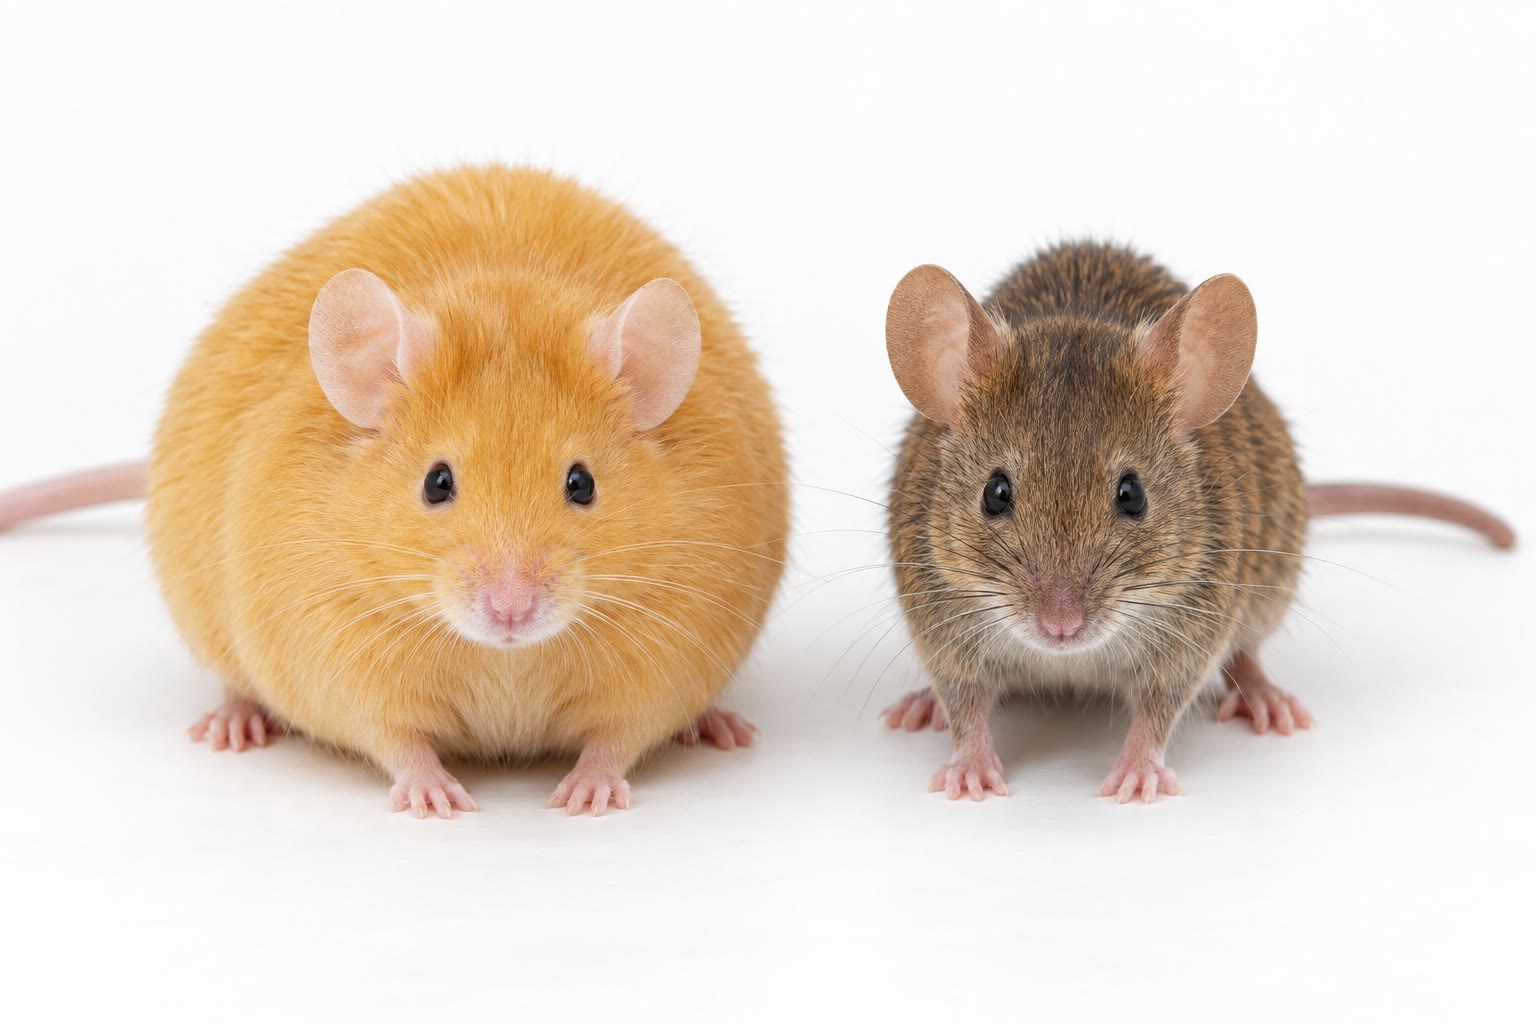
\includegraphics[width=0.62\linewidth]{images/book5/ai/b5-01-agouti-mice.jpg}

{\small Dois irmãos de ninhada $A^{vy}$ de genótipo idêntico: um
camundongo amarelo e obeso, no qual o transpóson a montante do
\emph{agouti} está não metilado, e um pardo pseudoagouti, no qual ele
está metilado.}
\end{omfigure}

\begin{proposition}[Onde se encontram estados epigenéticos hereditários]\label{prop:b3:chromatin-epigenetics:examples}
\index{variegação por efeito de posição}\index{vernalização}\index{paramutação}
Três sistemas bem analisados ilustram os mecanismos acima. A
\emph{\omterm{prop:b3:chromatin-epigenetics:examples}{variegação por efeito de posição}} em \emph{Drosophila}: um gene
deslocado por um rearranjo cromossômico para junto da \omterm{def:b3:chromatin-epigenetics:nucleosome}{heterocromatina}
é silenciado em algumas células e não em outras, o que dá um olho
mosqueado; cada mancha é um clone, o silenciamento se propaga a partir
da \omterm{def:b3:chromatin-epigenetics:nucleosome}{heterocromatina} pela alça da HP1, e os genes cuja mutação suprime a
variegação (genes \emph{Su(var)}) são a HP1 e a metiltransferase da
H3K9. A \emph{vernalização} em \emph{Arabidopsis}: semanas de frio de
inverno silenciam o repressor do florescimento \emph{FLC} pela
H3K27me3 depositada pelo Polycomb, o silêncio se mantém ao longo de
meses de crescimento primaveril e de milhares de divisões celulares, e
é reiniciado a cada geração, de modo que cada planta precisa passar
pelo seu próprio inverno. A \emph{paramutação} no milho: um alelo do
gene de pigmento \emph{b1}, quando encontra um outro alelo particular
num heterozigoto, converte-o ao seu próprio estado silencioso, e o
alelo convertido passa o estado a seus descendentes por gerações,
através de uma metilação dirigida por RNA pequeno retomada no
\cref{ch:b3:rna-regulation}. Em cada caso a herança é mitótica e
robusta; a transmissão entre gerações é ou ativamente reiniciada
(plantas) ou parcial e imperfeita (camundongos).
\end{proposition}

\begin{remark}[Os limites das alegações transgeracionais]\label{rem:b3:chromatin-epigenetics:limits}
Alegações de que a fome ou o estresse de um avô é ``herdado
epigeneticamente'' pelos netos humanos são comuns e em sua maioria não
comprovadas. Duas ondas de apagamento se interpõem entre uma marca
somática e um neto, os genes sob imprinting e alguns poucos
transpósons são os únicos sobreviventes documentados do apagamento em
mamíferos, e em coortes humanas os efeitos de um ambiente
compartilhado, do ambiente uterino e de diferenças genéticas são
difíceis de separar de uma marca carregada na linhagem germinativa. Os
casos demonstrados --- o $A^{vy}$, alguns \omterm{def:b3:chromatin-epigenetics:epigenetics}{epialelos} ligados a
transpósons, estados mediados por RNA em vermes e plantas --- são
reais, molecularmente compreendidos e restritos. O teorema deste
capítulo diz por quê: sem uma retroalimentação que empurre $\mu$ para
$1$, uma marca esquece a si mesma em poucas dezenas de divisões, e a
linhagem germinativa ainda acrescenta um reinício ativo.
\end{remark}

\section{Exercícios}

\begin{exercise}[$\star$]\label{exo:b3:chromatin-epigenetics:1}
Dê a composição de uma partícula do cerne do \omterm{def:b3:chromatin-epigenetics:nucleosome}{nucleossomo}, o
comprimento de DNA que ela liga e o comprimento típico do ligante. Por
que a digestão da \omterm{def:b3:chromatin-epigenetics:nucleosome}{cromatina} por nuclease deu uma escada de fragmentos
em vez de um rastro contínuo?
\end{exercise}

\begin{exercise}[$\star$]\label{exo:b3:chromatin-epigenetics:2}
O genoma de um sapo tem $3.0\times 10^{9}$ pares de bases por conjunto
haploide. Quantos \omterm{def:b3:chromatin-epigenetics:nucleosome}{nucleossomos} contém um núcleo diploide, tomando uma
repetição de \qty{190}{bp}, e qual é o comprimento de seu DNA?
\end{exercise}

\begin{exercise}[$\star$]\label{exo:b3:chromatin-epigenetics:3}
Decifre H3K27me3, H4K16ac e H3S10ph. Para cada um, diga se está
associado a \omterm{def:b3:chromatin-epigenetics:nucleosome}{cromatina} ativa ou silenciosa, e nomeie um \omterm{def:b3:chromatin-epigenetics:histone-code}{leitor} do
primeiro.
\end{exercise}

\begin{exercise}[$\star$]\label{exo:b3:chromatin-epigenetics:4}
Explique por que uma gata tricolor é quase sempre fêmea, e o que um
tricolor macho tem de ser.
\end{exercise}

\begin{exercise}[$\star\star$]\label{exo:b3:chromatin-epigenetics:5}
Calcule a \omterm{prop:b3:chromatin-epigenetics:compaction}{razão de empacotamento} da fibra de \qty{10}{nm} a partir dos
números da \cref{def:b3:chromatin-epigenetics:nucleosome} (repetição
\qty{200}{bp}, conta \qty{11}{nm}), e a razão necessária para caber os
\qty{4}{cm} de DNA de um cromossomo humano médio numa cromátide
mitótica de \qty{4}{\micro m}. Por qual fator adicional a fibra deve
ser dobrada?
\end{exercise}

\begin{exercise}[$\star\star$]\label{exo:b3:chromatin-epigenetics:6}
No modelo do \cref{thm:b3:chromatin-epigenetics:maintenance} com
$\mu = 0.98$ e $\delta = 0.01$, determine $p^{*}$ e o número de
divisões após o qual um sítio que começou metilado perdeu metade de
seu excesso sobre $p^{*}$. Repita para $\mu = 0.999$, $\delta = 0.001$.
\end{exercise}

\begin{exercise}[$\star\star$]\label{exo:b3:chromatin-epigenetics:7}
Um experimento de ChIP-seq em células de fígado dá um pico de H3K4me3
e um pico de H3K27ac no promotor do gene $A$, um amplo domínio de
H3K27me3 sobre o gene $B$ e H3K9me3 sobre o gene $C$. Preveja o estado
transcricional de cada um, e diga qual entre $B$ e $C$ tem mais chance
de ser ligado em outro tipo celular, e por quê.
\end{exercise}

\begin{exercise}[$\star\star$]\label{exo:b3:chromatin-epigenetics:8}
Uma mulher é portadora de uma deleção da região \emph{UBE3A} num dos
cromossomos 15, mas é saudável. Seu pai era portador da mesma deleção
e também era saudável. De qual síndrome, se alguma, cada um de seus
filhos corre risco, e com que probabilidade? E se a deleção tivesse
vindo da mãe dela?
\end{exercise}

\begin{exercise}[$\star\star$]\label{exo:b3:chromatin-epigenetics:9}
Preveja a consequência, num embrião de camundongo fêmea, de deletar o
gene \emph{\omterm{def:b3:chromatin-epigenetics:x-inactivation}{Xist}} de um dos cromossomos X; dos dois. Preveja o que um
transgene \emph{\omterm{def:b3:chromatin-epigenetics:x-inactivation}{Xist}} inserido num autossomo faz a esse autossomo.
\end{exercise}

\begin{exercise}[$\star\star\star$]\label{exo:b3:chromatin-epigenetics:10}
Explique, com o \cref{ex:b3:chromatin-epigenetics:cpg-deficit}, por
que as \omterm{def:b3:chromatin-epigenetics:methylation}{ilhas CpG} conservaram seus \omterm{def:b3:chromatin-epigenetics:methylation}{CpGs} enquanto o resto do genoma
perdeu quatro quintos deles, e o que isso implica sobre o estado de
metilação das ilhas na linhagem germinativa ao longo do tempo
evolutivo. Por que o argumento falha para um gene metilado apenas no
fígado?
\end{exercise}

\begin{exercise}[$\star\star\star$]\label{exo:b3:chromatin-epigenetics:11}
Mostre, usando a alça escritor--leitor da
\cref{prop:b3:chromatin-epigenetics:readers}, como um domínio de
H3K9me3 pode ser estável através da replicação embora cada divisão
dilua as \omterm{def:b3:chromatin-epigenetics:nucleosome}{histonas} marcadas pela metade com \omterm{def:b3:chromatin-epigenetics:nucleosome}{histonas} novas sem marca. O
que determina onde o domínio para de se propagar? Proponha um
experimento para testar sua explicação.
\end{exercise}

\begin{exercise}[$\star\star\star$]\label{exo:b3:chromatin-epigenetics:12}
Um estudo relata que os netos de pessoas que passaram por uma fome têm
metilação alterada num gene de crescimento e maior massa corporal.
Liste as explicações alternativas que precisam ser excluídas antes de
concluir que uma marca de metilação foi transmitida pela linhagem
germinativa, e diga que experimento em camundongos resolveria a
questão.
\end{exercise}

\section{Problema: a memória de um gene silenciado}

\begin{problem}[{Problema de fim de semana --- um genoma humano
acondicionado em seu núcleo, uma marca de metilação acompanhada ao
longo das divisões, uma gata tricolor lida como mapa clonal e as
doenças de uma região sob imprinting contadas, terminando no número de
divisões que uma marca sobrevive sem retroalimentação e no tamanho da
população de células que escolheu seu X}]
\label{pb:b3:chromatin-epigenetics:1}
Dados: um núcleo diploide humano contém $6.4\times 10^{9}$ pares de
bases, a \qty{0.34}{nm} e \qty{650}{Da} por par; a repetição do
\omterm{def:b3:chromatin-epigenetics:nucleosome}{nucleossomo} é de \qty{200}{bp}, um octâmero de \omterm{def:b3:chromatin-epigenetics:nucleosome}{histonas} pesa
\qty{108}{kDa} e uma partícula do cerne é um disco de \qty{11}{nm} de
diâmetro e \qty{5.5}{nm} de espessura. O núcleo é uma esfera de
\qty{10}{\micro m} de diâmetro. O genoma tem \qty{42}{\%} de G$+$C.
Metilação num \omterm{def:b3:chromatin-epigenetics:methylation}{CpG} comum: $\mu = 0.99$, $\delta = 0.02$ por divisão.

\medskip
\noindent\textbf{Parte I --- O empacotamento.}
\begin{enumerate}
  \item Calcule o comprimento total de DNA no núcleo e o número de
        \omterm{def:b3:chromatin-epigenetics:nucleosome}{nucleossomos}.
  \item Calcule a massa total de \omterm{def:b3:chromatin-epigenetics:nucleosome}{histonas} (apenas os octâmeros) e a de
        DNA, em picogramas ($\qty{1}{Da} = \qty{1.66e-24}{g}$).
  \item Calcule o volume do núcleo e o volume total das partículas do
        cerne, tratadas como cilindros. Que fração do núcleo elas
        preenchem?
  \item Se os \omterm{def:b3:chromatin-epigenetics:nucleosome}{nucleossomos} fossem dispostos ponta a ponta como uma
        fibra de \qty{10}{nm}, qual seria o comprimento da fibra e
        qual a \omterm{prop:b3:chromatin-epigenetics:compaction}{razão de empacotamento} em relação ao DNA nu?
  \item A fibra é dobrada em alças de \qty{200}{kb} ancoradas pela
        coesina. Quantas alças, e quantos \omterm{def:b3:chromatin-epigenetics:nucleosome}{nucleossomos} por alça?
  \item Sob a hipótese de independência, quantos dinucleotídeos \omterm{def:b3:chromatin-epigenetics:methylation}{CpG} o
        genoma diploide conteria? O número observado é
        $5.6\times 10^{7}$. Que fração se perdeu, e por qual
        mecanismo mutacional?
\end{enumerate}

\medskip
\noindent\textbf{Parte II --- Uma marca ao longo das divisões.}
\begin{enumerate}[resume]
  \item Escreva a recorrência de $p_{n}$ e calcule $p^{*}$.
  \item Um \omterm{def:b3:chromatin-epigenetics:methylation}{CpG} de promotor está totalmente metilado em $n = 0$.
        Calcule $p_{n}$ após $10$, $50$ e $200$ divisões.
  \item Após quantas divisões o excesso $p_{n} - p^{*}$ cai pela
        metade? Uma célula-tronco tecidual se divide cerca de uma vez
        por semana: quantos anos são esses?
  \item Um fármaco inibe completamente a \omterm{def:b3:chromatin-epigenetics:methylation}{DNMT1} ($\mu = 0$) e também a
        DNMT3 ($\delta = 0$). Mostre que a fração de fitas metiladas
        na população cai pela metade a cada divisão, e determine o
        número de divisões para levar \qty{80}{\%} de metilação a
        menos de \qty{5}{\%}.
  \item Numa ilha silenciada os \omterm{def:b3:chromatin-epigenetics:histone-code}{leitores} de \omterm{def:b3:chromatin-epigenetics:methylation}{metil-CpG} recrutam a
        metilação da H3K9, que recruta a DNMT3, de modo que dentro da
        ilha $\mu = 0.9995$ e $\delta = 0.0005$. Recalcule a
        meia-vida do excesso, em divisões e em anos a uma divisão por
        semana.
  \item Explique numa frase por que é o resultado da questão 11, e não
        o da questão 9, o que um gene silenciado por toda a vida
        exige, e que tipo de arranjo molecular o produz.
\end{enumerate}

\medskip
\noindent\textbf{Parte III --- O mapa da gata tricolor.}
\begin{enumerate}[resume]
  \item Uma gata é heterozigótica para o gene alaranjado ligado ao X.
        Explique por que sua pelagem tem manchas alaranjadas e pretas
        e o que representa uma mancha.
  \item A \omterm{def:b3:chromatin-epigenetics:x-inactivation}{inativação do X} ocorreu quando as células destinadas a
        formar a pele eram $N$. Cada uma escolheu um X ao acaso. Qual
        é a probabilidade de todas as $N$ terem escolhido o mesmo, o
        que daria uma gata de cor única?
  \item Nenhuma heterozigota de cor única foi documentada entre talvez
        um bilhão de gatas; tome a probabilidade como $10^{-9}$ e
        estime $N$.
  \item A superfície da pele da gata é de cerca de \qty{0.3}{m^2} e
        suas manchas têm em média \qty{15}{cm^2}. Estime o número de
        manchas e explique por que ele é maior que $N$.
  \item Um gato XXY também é tricolor. Quantos \omterm{def:b3:chromatin-epigenetics:x-inactivation}{corpúsculos de Barr}
        exibem suas células? Quantos numa fêmea XXX e num macho XY?
  \item Um gene que escapa da inativação está presente em duas cópias
        ativas nas fêmeas e em uma nos machos. Dê uma razão pela qual
        esse escape pode ser tolerado e uma situação em que ele
        importa.
\end{enumerate}

\medskip
\noindent\textbf{Parte IV --- O cromossomo 15.}
\begin{enumerate}[resume]
  \item A síndrome de Prader--Willi afeta cerca de um nascimento em
        \num{15000}; \qty{70}{\%} dos casos são uma deleção de novo do
        15q11--q13 paterno e \qty{25}{\%} uma \omterm{def:b3:chromatin-epigenetics:imprinting}{dissomia uniparental}
        materna. Calcule a frequência de nascimento de cada causa.
  \item A síndrome de Angelman tem mais ou menos a mesma frequência;
        \qty{70}{\%} são deleções maternas, \qty{5}{\%} dissomias
        paternas e \qty{10}{\%} mutações pontuais do \emph{UBE3A}. Por
        que as mutações pontuais são uma causa de Angelman, mas quase
        nunca de Prader--Willi?
  \item Um pai é portador de uma translocação balanceada que dá a
        \qty{20}{\%} de seus espermatozoides uma deleção 15q11--q13.
        Que fração de seus filhos tem Prader--Willi, e que fração
        Angelman?
  \item A \omterm{def:b3:chromatin-epigenetics:imprinting}{dissomia uniparental} surge quando um zigoto trissômico perde
        um cromossomo. Se um zigoto com trissomia do 15 perde ao acaso
        um de seus três cromossomos, e a trissomia veio da mãe (duas
        cópias maternas), qual é a probabilidade de o sobrevivente ter
        dissomia materna? Qual síndrome?
  \item Os genes de Prader--Willi são de expressão paterna e o gene de
        Angelman, de expressão materna. Usando a teoria do parentesco,
        diga quais dos sintomas das duas síndromes (dificuldade de
        alimentação ao nascer contra apetite voraz) se encaixam na
        teoria e quais são mais difíceis de encaixar.
  \item Propõe-se um método de tratar a síndrome de Angelman
        reativando o \emph{UBE3A} paterno silencioso. Seu silêncio se
        deve a um RNA antissenso de expressão paterna. Proponha o alvo
        molecular e diga por que a terapia não perturbaria os outros
        genes sob imprinting.
  \item Resuma: a meia-vida de uma marca sem retroalimentação
        (questão~9) e com ela (questão~11), em divisões; e a população
        fundadora $N$ da pelagem tricolor (questão~15).
\end{enumerate}
\end{problem}
